\subsection{Use case}
\begin{figure}[!h]
	\centering
	\makebox[\textwidth][c]{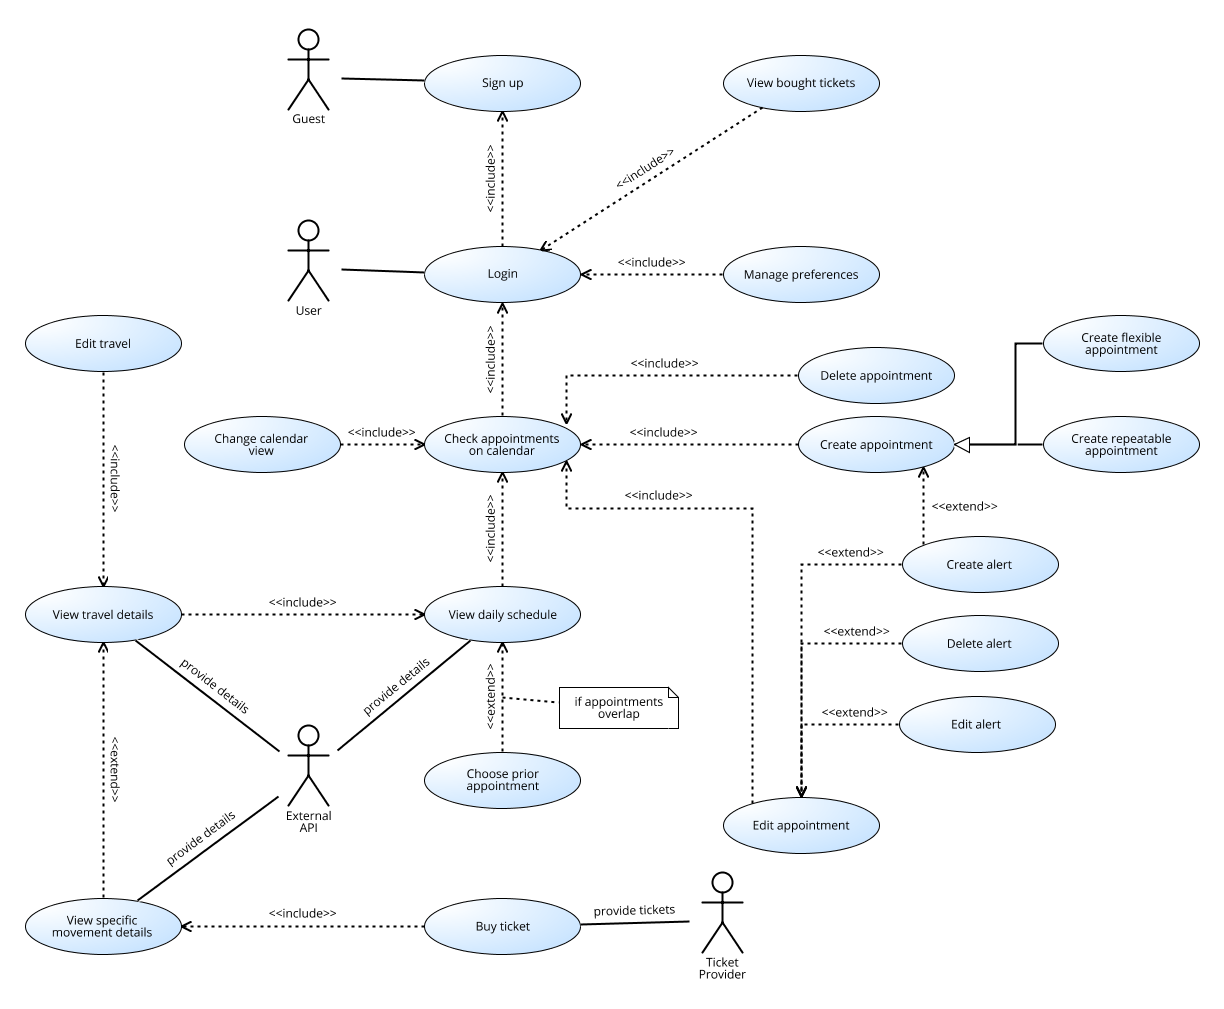
\includegraphics[width=1.2\textwidth]{Images/UseCaseDiagram.png}}%
\end{figure}
\clearpage

\subsubsection{Sign up}
\begin{table}[!h]
	\centering
	{\renewcommand{\arraystretch}{2}%
		\begin{tabular}{|l|p{12cm}|}
			\hline
			\textbf{Name} 				& \textbf{Sign up} \\ \hline
			\textbf{Actors} 			& Guest \\ \hline
			\textbf{Entry conditions} 	& The guest is on the log in page of the application and clicks on “Register” button. \\ \hline
			\textbf{Flow of events}		& \begin{minipage}[t]{0.75\textwidth}
				\begin{enumerate}
					\item A pop-up shows up asking to the guest if he wants to connect an existing account, such as Google or Facebook, or if he want to create a new account.
					\begin{enumerate}
						\item If the guest connects his account, the system accepts the request and creates a new Travlendar+ account based on provided account.
						\item If the guest chooses to create a new account, he is redirected to the registration page which contains all the fields to be filled.
					\end{enumerate}
					\item The guest fills out all the mandatory fields.
					\item (Optional) The guest adjusts the preferences settings.
					\item The guest clicks on button “Confirm”.
					\item The system checks data provided and eventually creates and registers the user account.
				\end{enumerate}
			\end{minipage}	\\ \hline
			\textbf{Exit conditions}	& The guest has successfully created a new account and he can log into the system with his credentials. \\ \hline
			\textbf{Exceptions}			& \begin{minipage}[t]{0.75\textwidth}
				\begin{itemize}
					\item Email provided is already in use. The system does not proceed in the registration process and the account is not created. It is possible to repeat the procedure.
					\item Data provided are incorrect. The system highlights the incorrect fields and asks the user to repeat the procedure.
				\end{itemize} 
			\end{minipage} \\ \hline
	\end{tabular}}
\end{table}
\clearpage

\subsubsection{Log in}
\begin{table}[!h]
	\centering
	{\renewcommand{\arraystretch}{2}%
		\begin{tabular}{|l|p{12cm}|}
			\hline
			\textbf{Name} 				& \textbf{Log in} \\ \hline
			\textbf{Actors} 			& User \\ \hline
			\textbf{Entry conditions} 	& The user launches the application and clicks on the “Log In” button. \\ \hline
			\textbf{Flow of events}		& \begin{minipage}[t]{0.75\textwidth}
				\begin{enumerate}
					\item The user inserts his email.
					\item The user inserts his password.
					\item The user clicks on the “Log In” button.
				\end{enumerate}
			\end{minipage}	\\ \hline
			\textbf{Exit conditions}	& The login procedure is successfully completed. The user is logged into the system and is able to access to all the functionalities. \\ \hline
			\textbf{Exceptions}			& The credentials provided are not associated to any existing account. The login procedure is rejected and the guest is brought back to the login page. It is possible to repeat the procedure. \\ \hline
	\end{tabular}}
\end{table}

\subsubsection{Manage preferences}
\begin{table}[!h]
	\centering
	{\renewcommand{\arraystretch}{2}%
		\begin{tabular}{|l|p{12cm}|}
			\hline
			\textbf{Name} 				& \textbf{Manage preferences} \\ \hline
			\textbf{Actors} 			& User \\ \hline
			\textbf{Entry conditions} 	& The user clicks on “Preferences” from the side menu on the homepage. \\ \hline
			\textbf{Flow of events}		& \begin{minipage}[t]{0.75\textwidth}
				\begin{enumerate}
					\item The system shows the preferences settings, that include transport means owned, favorite kind of travel and other advanced options.
					\item The user accesses to the desired settings and adjusts the preferences as wanted.
					\item The user saves the changes.
				\end{enumerate}
			\end{minipage}	\\ \hline
			\textbf{Exit conditions}	& The changes are saved and remembered from the system. The preferences have been updated.  \\ \hline
			\textbf{Exceptions}			& The user clicks on “back” without having confirmed the creation. The new preferences are not saved and the application returns to the homepage. It is possible to repeat the procedure. \\ \hline
	\end{tabular}}
\end{table}
\clearpage

\subsubsection{View daily schedule}
\begin{table}[!h]
	\centering
	{\renewcommand{\arraystretch}{2}%
		\begin{tabular}{|l|p{12cm}|}
			\hline
			\textbf{Name} 				& \textbf{View daily schedule} \\ \hline
			\textbf{Actors} 			& User, External APIs \\ \hline
			\textbf{Entry conditions} 	& The user clicks on the “View daily schedule” button while checking an appointment on his calendar. \\ \hline
			\textbf{Flow of events}		& \begin{minipage}[t]{0.75\textwidth}
				\begin{enumerate}
					\item The system receives data from different external APIs about routes, traffic, weather and available transport means and computes the best travel option according to the user preferences.
					\item The system provides a graphic overview of all the travels scheduled for the day, with the relative movements.
					\item The user checks all the information needed and eventually clicks on a specific travel or movement to get further information.
				\end{enumerate}
			\end{minipage}	\\ \hline
			\textbf{Exit conditions}	& User has obtained all the information needed and has clicked “back” to return to the homepage or has selected a specific travel/movement to get further information.  \\ \hline
			\textbf{Exceptions}			& \begin{minipage}[t]{0.75\textwidth}
				\begin{itemize}
					\item Some of the appointments overlap. The system is not able to compute travels between the appointments and forces the user to choose a prior appointment.
					\item Some of the appointments are not reachable in the allotted time. The system doesn’t show the travel and signals the problem to the user with a warning.
					\item Internet connection is not available. The system fails to compute the best travel option and displays a warning to the user.
				\end{itemize} 
			\end{minipage} \\ \hline
	\end{tabular}}
\end{table}
\clearpage

\subsubsection{View travel details}
\begin{table}[!h]
	\centering
	{\renewcommand{\arraystretch}{2}%
		\begin{tabular}{|l|p{12cm}|}
			\hline
			\textbf{Name} 				& \textbf{View travel details} \\ \hline
			\textbf{Actors} 			& User, External APIs \\ \hline
			\textbf{Entry conditions} 	& The user is checking his daily schedule and clicks on a specific travel. \\ \hline
			\textbf{Flow of events}		& \begin{minipage}[t]{0.75\textwidth}
				\begin{enumerate}
					\item The system receives data from different external APIs and collects detailed information about the travel, such as the specific itinerary on the map and the weather conditions.
					\item The user is redirected to a new page that displays all the information about the selected travel.
					\item The user checks all the information needed and eventually clicks on a specific movement to get further information or buy a ticket.
				\end{enumerate}
			\end{minipage}	\\ \hline
			\textbf{Exit conditions}	& User has obtained all the information needed and has clicked “back” to return to the daily schedule or has selected a specific movement to get further information.  \\ \hline
			\textbf{Exceptions}			& Internet connection is not available. The system fails to obtain the needed information and displays a warning to the user.  \\ \hline
	\end{tabular}}
\end{table}

\subsubsection{Edit travel}
\begin{table}[!h]
	\centering
	{\renewcommand{\arraystretch}{2}%
		\begin{tabular}{|l|p{12cm}|}
			\hline
			\textbf{Name} 				& \textbf{Edit travel} \\ \hline
			\textbf{Actors} 			& User \\ \hline
			\textbf{Entry conditions} 	& The user is checking a specific travel. \\ \hline
			\textbf{Flow of events}		& \begin{minipage}[t]{0.75\textwidth}
				\begin{enumerate}
					\item The user provides modifications to the travel as followed:
					\begin{enumerate}
						\item Clicking on the travel preferences and switching to a different alternative.
						\item Clicking on a specific movement and changing the transport mean.
					\end{enumerate}
					\item The user saves the changes.
				\end{enumerate}
			\end{minipage}	\\ \hline
			\textbf{Exit conditions}	& The changes are saved and the system displays the new modified travel.   \\ \hline
			\textbf{Exceptions}			& There are no possible alternatives for the selected travel. The system displays a warning to notify the user.  \\ \hline
	\end{tabular}}
\end{table}

\subsubsection{View specific movement details}
\begin{table}[!h]
	\centering
	{\renewcommand{\arraystretch}{2}%
		\begin{tabular}{|l|p{12cm}|}
			\hline
			\textbf{Name} 				& \textbf{View specific movement details} \\ \hline
			\textbf{Actors} 			& User \\ \hline
			\textbf{Entry conditions} 	& User is checking a specific travel and select a specific movement. \\ \hline
			\textbf{Flow of events}		& \begin{minipage}[t]{0.75\textwidth}
				\begin{enumerate}
					\item The system receives data from different external APIs and collects detailed information about the movement, such as the specific itinerary on the map, the weather conditions and the eventual availability of tickets.
					\item The user is redirected to a new page that displays all the information about the selected movement.
					\item The user checks all the information needed and eventually proceeds in buying a ticket.
				\end{enumerate}
			\end{minipage}	\\ \hline
			\textbf{Exit conditions}	& User has obtained all the information needed and has clicked “back” to return to the travel page or has proceeded in buying a ticket.  \\ \hline
			\textbf{Exceptions}			& Internet connection is not available. The system fails to obtain the needed information and displays a warning to the user.  \\ \hline
	\end{tabular}}
\end{table}

\subsubsection{Choose prior appointment}
\begin{table}[!h]
	\centering
	{\renewcommand{\arraystretch}{2}%
		\begin{tabular}{|l|p{12cm}|}
			\hline
			\textbf{Name} 				& \textbf{Choose prior appointment} \\ \hline
			\textbf{Actors} 			& User \\ \hline
			\textbf{Entry conditions} 	& The user is checking the schedule and two appointments overlap. \\ \hline
			\textbf{Flow of events}		& \begin{minipage}[t]{0.75\textwidth}
				\begin{enumerate}
					\item The system signals the user the exactly time overlapping of the appointments.
					\item The user clicks on the preferred appointment.
					\item The system re-computes the daily schedule giving priority to the chosen appointment.
				\end{enumerate}
			\end{minipage}	\\ \hline
			\textbf{Exit conditions}	& No more appointments overlap. The system shows the daily schedule without errors.  \\ \hline
			\textbf{Exceptions}			& No exceptions expected  \\ \hline
	\end{tabular}}
\end{table}
\clearpage

\subsubsection{Buy ticket}
\begin{table}[!h]
	\centering
	{\renewcommand{\arraystretch}{2}%
		\begin{tabular}{|l|p{12cm}|}
			\hline
			\textbf{Name} 				& \textbf{Buy ticket} \\ \hline
			\textbf{Actors} 			& User, Ticket provider \\ \hline
			\textbf{Entry conditions} 	& User is checking a specific movement and clicks on “Buy ticket” \\ \hline
			\textbf{Flow of events}		& \begin{minipage}[t]{0.75\textwidth}
				\begin{enumerate}
					\item The system connects trough APIs to the external system of the ticket provider.
					\item The system shows the user a form to fill with all the payment information.
					\item The user fills out all the fields and confirm the payment.
					\item The system sends information to the ticket provider and waits for confirmation and ticket data.
				\end{enumerate}
			\end{minipage}	\\ \hline
			\textbf{Exit conditions}	& Payment is successfully fulfilled and bought tickets are available for the view. The user is brought back to the movement page.  \\ \hline
			\textbf{Exceptions}			& \begin{minipage}[t]{0.75\textwidth}
				\begin{itemize}
					\item Payment is rejected. The system notifies the user with a warning. It is possible to repeat the procedure. 
					\item Internet connection is not available. The system fails to connect to the ticket provider and notifies the user with a warning. The application returns to the movement page.
				\end{itemize} 
			\end{minipage} \\ \hline
	\end{tabular}}
\end{table}
\clearpage

\subsubsection{Delete appointment}
\begin{table}[!h]
	\centering
	{\renewcommand{\arraystretch}{2}%
		\begin{tabular}{|l|p{12cm}|}
			\hline
			\textbf{Name} 				& \textbf{Delete appointment} \\ \hline
			\textbf{Actors} 			& User \\ \hline
			\textbf{Entry conditions} 	& The user selects a specific appointment in his calendar (through daily or weekly view) and clicks on “Delete” button. \\ \hline
			\textbf{Flow of events}		& \begin{minipage}[t]{0.75\textwidth}
				\begin{enumerate}
					\item A pop-up shows up, asking the user to confirm the deletion.
					\item The user confirms the deletion.
					\item The system removes all the appointment information from the memory, alert included.
				\end{enumerate}
			\end{minipage}	\\ \hline
			\textbf{Exit conditions}	& The appointment has been deleted and removed from the system. The user is redirected to his calendar page, which has been updated with the removal of the appointment.  \\ \hline
			\textbf{Exceptions}			& The user does not confirm the deletion. The appointment has not been deleted and the user is redirected to his calendar page. It is possible to repeat the procedure.  \\ \hline
	\end{tabular}}
\end{table}
\clearpage

\subsubsection{Create appointment}
\begin{table}[!h]
	\centering
	{\renewcommand{\arraystretch}{2}%
		\begin{tabular}{|l|p{12cm}|}
			\hline
			\textbf{Name} 				& \textbf{Create appointment} \\ \hline
			\textbf{Actors} 			& User \\ \hline
			\textbf{Entry conditions} 	& The user is checking his calendar and clicks on “Create appointment” button. \\ \hline
			\textbf{Flow of events}		& \begin{minipage}[t]{0.75\textwidth}
				\begin{enumerate}
					\item The user is redirected to the appointment creation page, which contains all the fields required to perform the creation.
					\item The user fills out all mandatory fields.
					The following steps aren’t mandatory:
					\begin{enumerate}
						\item User chooses among the available icons.
						\item User adds an alert to remember the appointment.
						\item User clicks on “More options” and provides more detailed options.
					\end{enumerate}
					\item User confirms the creation.
					\item The system saves the appointment information.
				\end{enumerate}
			\end{minipage}	\\ \hline
			\textbf{Exit conditions}	& The appointment is created and inserted in the system. The user is redirected to his calendar page, which has been updated with the new appointment.  \\ \hline
			\textbf{Exceptions}			& \begin{minipage}[t]{0.75\textwidth}
				\begin{itemize}
					\item The user has provided incorrect information: the appointment is not created and the user must repeat the procedure. 
					\item The user clicks on “back” without having confirmed the creation. The appointment is not created and the application returns to the calendar page. It is possible to repeat the procedure.
					\item The appointment overlaps with other previously created appointments. The appointment is created and inserted anyway, but the user receives a notification of the overlapping.
				\end{itemize} 
			\end{minipage} \\ \hline
	\end{tabular}}
\end{table}
\clearpage

\subsubsection{Edit appointment}
\begin{table}[!h]
	\centering
	{\renewcommand{\arraystretch}{2}%
		\begin{tabular}{|l|p{12cm}|}
			\hline
			\textbf{Name} 				& \textbf{Edit appointment} \\ \hline
			\textbf{Actors} 			& User \\ \hline
			\textbf{Entry conditions} 	& The user selects a specific appointment in his calendar (through daily or weekly view) and clicks on “Edit” button. \\ \hline
			\textbf{Flow of events}		& \begin{minipage}[t]{0.75\textwidth}
				\begin{enumerate}
					\item The user is redirected to the appointment editing page which contains all the previously inserted information.
					\item The user can perform the following actions:
					\begin{enumerate}
						\item Changing the appointment icon.
						\item Editing the information.
						\item Adding an alert to the appointment.
						\item Clicking on “More options” and providing more detailed options.
					\end{enumerate}
					\item The user saves the changes.
					\item The system saves the updated appointment information.
				\end{enumerate}
			\end{minipage}	\\ \hline
			\textbf{Exit conditions}	& The changes are saved and the appointment has been modified. The user is redirected to his calendar page, which has been updated with the new information provided.  \\ \hline
			\textbf{Exceptions}			& \begin{minipage}[t]{0.75\textwidth}
				\begin{itemize}
					\item The user has provided incorrect information: the changes are not saved and the user must repeat the procedure. 
					\item The user clicks on “back” without having saved the changes. The appointment has not been modified and the application returns to the calendar page. It is possible to repeat the procedure.
					\item The appointment now overlaps with other previously created appointments. The changes as saved anyway, but the user receives a notification of the overlapping.
				\end{itemize} 
			\end{minipage} \\ \hline
	\end{tabular}}
\end{table}
\clearpage

\subsubsection{Create flexible appointment}
\begin{table}[!h]
	\centering
	{\renewcommand{\arraystretch}{2}%
		\begin{tabular}{|l|p{12cm}|}
			\hline
			\textbf{Name} 				& \textbf{Create flexible appointment} \\ \hline
			\textbf{Actors} 			& User \\ \hline
			\textbf{Entry conditions} 	& The user is creating/editing an appointment, clicks on “More options” and clicks on the “Flexible” field. \\ \hline
			\textbf{Flow of events}		& \begin{minipage}[t]{0.75\textwidth}
				\begin{enumerate}
					\item A pop-up shows up, containing the fields to be filled.
					\item The user fills out the fields, specifying the time range of the appointment.
					\item The user confirms the choice.
				\end{enumerate}
			\end{minipage}	\\ \hline
			\textbf{Exit conditions}	& The choice is saved for later and the user is back on the More option page. At the end of the creation process, the appointment will be created at a time compatible with the time interval provided.  \\ \hline
			\textbf{Exceptions}			& The user clicks on “back” without having confirmed the choice. The appointment has not been modified and the application returns to the More options page. It is possible to repeat the procedure.  \\ \hline
	\end{tabular}}
\end{table}

\subsubsection{Create repeatable appointment}
\begin{table}[!h]
	\centering
	{\renewcommand{\arraystretch}{2}%
		\begin{tabular}{|l|p{12cm}|}
			\hline
			\textbf{Name} 				& \textbf{Create repeatable appointment} \\ \hline
			\textbf{Actors} 			& User \\ \hline
			\textbf{Entry conditions} 	& The user is creating/editing an appointment, clicks on “More options” and clicks on the “Flexible” field. \\ \hline
			\textbf{Flow of events}		& \begin{minipage}[t]{0.75\textwidth}
				\begin{enumerate}
					\item A pop-up shows up, containing the fields to be filled.
					\item The user fills out the fields, specifying the days in which the appointment is wanted to be created.
					\item The user confirms the choice.
				\end{enumerate}
			\end{minipage}	\\ \hline
			\textbf{Exit conditions}	& The choice is saved for later and the user is back on the More option page. The appointment is now a repeatable appointment.  \\ \hline
			\textbf{Exceptions}			& The user clicks on “back” without having confirmed the choice. The appointment has not been modified and the application returns to the More options page. It is possible to repeat the procedure.  \\ \hline
	\end{tabular}}
\end{table}
\clearpage

\subsubsection{Create alert}
\begin{table}[!h]
	\centering
	{\renewcommand{\arraystretch}{2}%
		\begin{tabular}{|l|p{12cm}|}
			\hline
			\textbf{Name} 				& \textbf{Create alert} \\ \hline
			\textbf{Actors} 			& User \\ \hline
			\textbf{Entry conditions} 	& The user is on the appointment creation/editing page and clicks on the “Add alert” button. \\ \hline
			\textbf{Flow of events}		& \begin{minipage}[t]{0.75\textwidth}
				\begin{enumerate}
					\item The user is redirected to the alert creation/editing page.
					\item The user fills the field specifying the time of the alert.
					\item The user confirms the creation.
					\item The system saves the alert information.
				\end{enumerate}
			\end{minipage}	\\ \hline
			\textbf{Exit conditions}	&The alert has been created and inserted in the system. The application returns to the appointment creation/editing page and it is now possible to edit the alert. \\ \hline
			\textbf{Exceptions}			& The user clicks on “back” without having confirmed the creation. The alert is not created and the application returns to the event creation page. It is possible to repeat the procedure.  \\ \hline
	\end{tabular}}
\end{table}
\clearpage

\subsubsection{Edit alert}
\begin{table}[!h]
	\centering
	{\renewcommand{\arraystretch}{2}%
		\begin{tabular}{|l|p{12cm}|}
			\hline
			\textbf{Name} 				& \textbf{Edit alert} \\ \hline
			\textbf{Actors} 			& User \\ \hline
			\textbf{Entry conditions} 	& The user is on the appointment creation/editing page and clicks on the “Edit alert” button. \\ \hline
			\textbf{Flow of events}		& \begin{minipage}[t]{0.75\textwidth}
				\begin{enumerate}
					\item The user is redirected to the alert creation/editing page.
					\item The user replaces needed information with updated ones. 
					\item The user saves the changes.
					\item The system saves the alert information.
				\end{enumerate}
			\end{minipage}	\\ \hline
			\textbf{Exit conditions}	& All the changes have been saved and inserted in the system. The application returns to the appointment creation/editing page and it is possible to repeat the procedure.  \\ \hline
			\textbf{Exceptions}			& The user clicks on “back” without having saved the changes. The changes have not been saved and the application returns to the appointment creation/modification page. It is possible to repeat the procedure.  \\ \hline
	\end{tabular}}
\end{table}
\clearpage

\subsubsection{Delete alert}
\begin{table}[!h]
	\centering
	{\renewcommand{\arraystretch}{2}%
		\begin{tabular}{|l|p{12cm}|}
			\hline
			\textbf{Name} 				& \textbf{Delete alert} \\ \hline
			\textbf{Actors} 			& User \\ \hline
			\textbf{Entry conditions} 	& The user is on the appointment creation/editing page and clicks on the “Edit alert” button. \\ \hline
			\textbf{Flow of events}		& \begin{minipage}[t]{0.75\textwidth}
				\begin{enumerate}
					\item The user is redirected to the alert creation/editing page.
					\item The user clicks on “Delete”. 
					\item The user confirms the deletion.
					\item The system removes all the alert information from the memory.
				\end{enumerate}
			\end{minipage}	\\ \hline
			\textbf{Exit conditions}	& The alert has been deleted and removed from the system. The application returns to the appointment creation/editing page and it is now possible to add a new alert.  \\ \hline
			\textbf{Exceptions}			& The user does not confirm the deletion. The alert has not been deleted and the application returns to the alert editing page. It is possible to repeat the procedure.  \\ \hline
	\end{tabular}}
\end{table}

\subsubsection{Check appointments on calendar}
\begin{table}[!h]
	\centering
	{\renewcommand{\arraystretch}{2}%
		\begin{tabular}{|l|p{12cm}|}
			\hline
			\textbf{Name} 				& \textbf{Check appointments on calendar} \\ \hline
			\textbf{Actors} 			& User \\ \hline
			\textbf{Entry conditions} 	& The user is logged in and he is on the homepage of the application. \\ \hline
			\textbf{Flow of events}		& \begin{minipage}[t]{0.75\textwidth}
				\begin{enumerate}
					\item The system shows an overview of the existing appointments.
					\item The user moves between the appointments and collects the needed infomation.
				\end{enumerate}
			\end{minipage}	\\ \hline
			\textbf{Exit conditions}	& The user has collected the needed information and moves to a different page.  \\ \hline
			\textbf{Exceptions}			& No exception expected.  \\ \hline
	\end{tabular}}
\end{table}
\clearpage

\subsubsection{Change calendar view}
\begin{table}[!h]
	\centering
	{\renewcommand{\arraystretch}{2}%
		\begin{tabular}{|l|p{12cm}|}
			\hline
			\textbf{Name} 				& \textbf{Change calendar view} \\ \hline
			\textbf{Actors} 			& User \\ \hline
			\textbf{Entry conditions} 	& The user is on the homepage of the application and he is checking his appointments. \\ \hline
			\textbf{Flow of events}		& \begin{minipage}[t]{0.75\textwidth}
				\begin{enumerate}
					\item The user opens the lateral menu.
					\item The user clicks on one of available view (daily, weekly or monthly).
					\item The system changes the layout according to the user’s choice. 
				\end{enumerate}
			\end{minipage}	\\ \hline
			\textbf{Exit conditions}	& The layout is changed and the user is back on the calendar view.  \\ \hline
			\textbf{Exceptions}			& No exception expected.  \\ \hline
	\end{tabular}}
\end{table}
\clearpage

\subsection{Sequence diagram}
\subsubsection{Guest registration}
\begin{figure}[!h]
	\centering
	\begin{minipage}[b]{0.75\textwidth}
		\makebox[\textwidth][c]{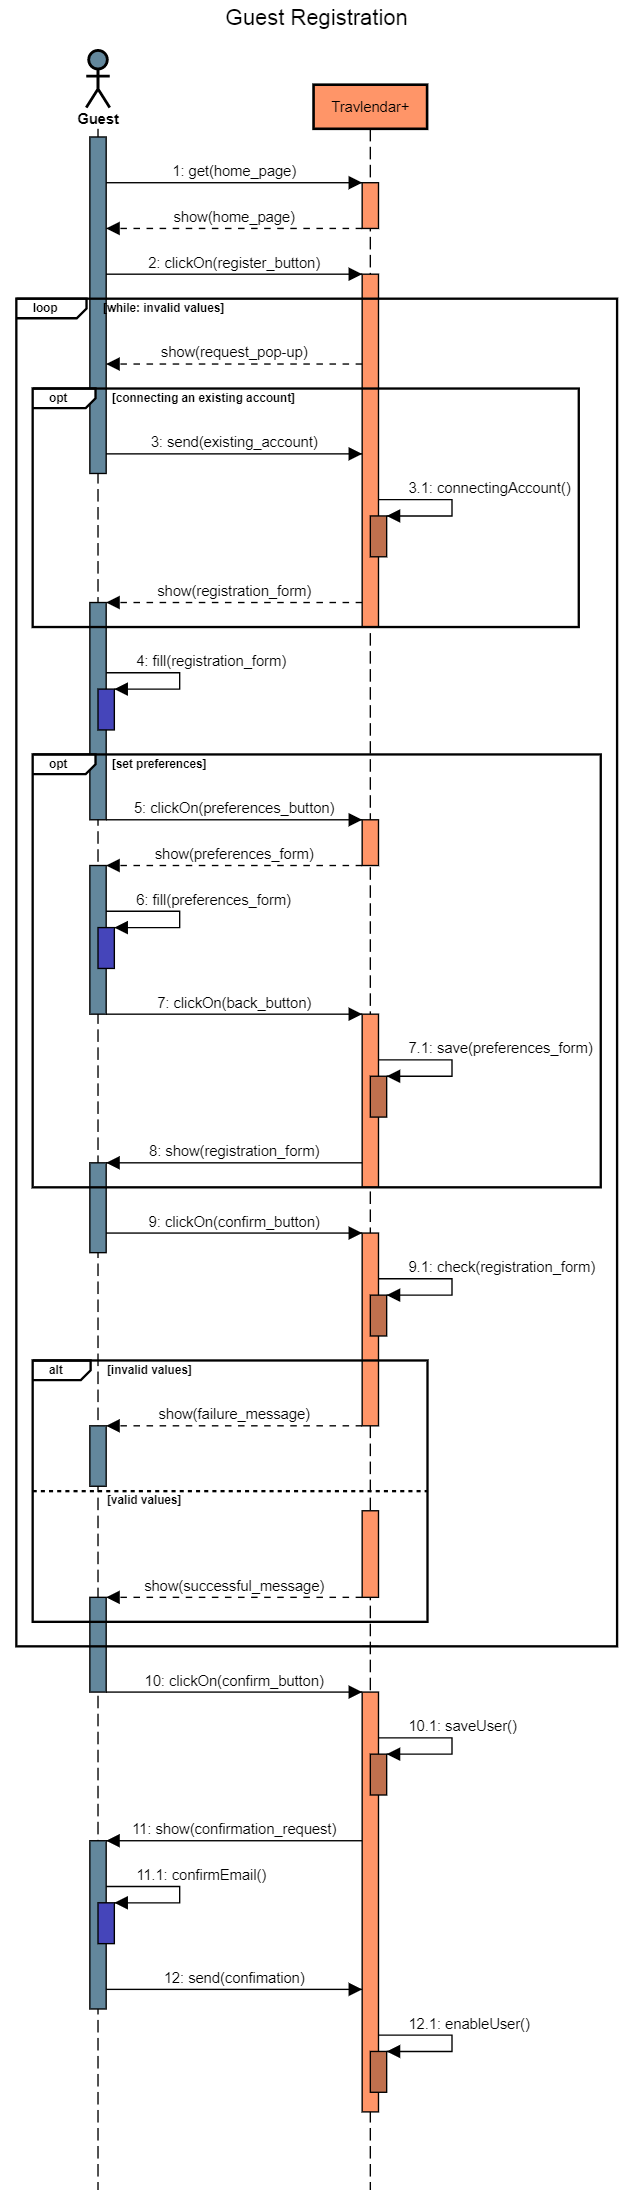
\includegraphics[width=0.50\textwidth]{Images/SequenceDiagram/GuestRegistration.png}}%
	\end{minipage}
\end{figure}
\clearpage

\subsubsection{User Login}
\begin{figure}[!h]
	\centering
	\begin{minipage}[b]{0.75\textwidth}
		\makebox[\textwidth][c]{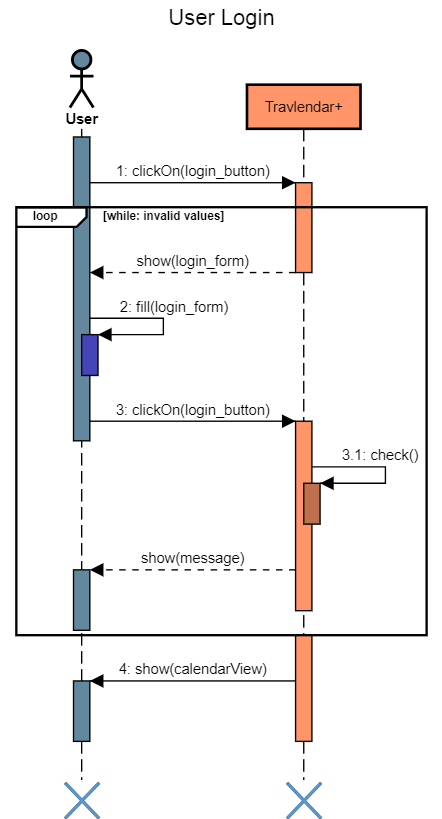
\includegraphics[width=0.50\textwidth]{Images/SequenceDiagram/UserLogin.png}}%
	\end{minipage}
\end{figure}
\clearpage

\subsubsection{Appointment creation}
\begin{figure}[!h]
	\centering
	\begin{minipage}[b]{0.65\textwidth}
		\makebox[\textwidth][c]{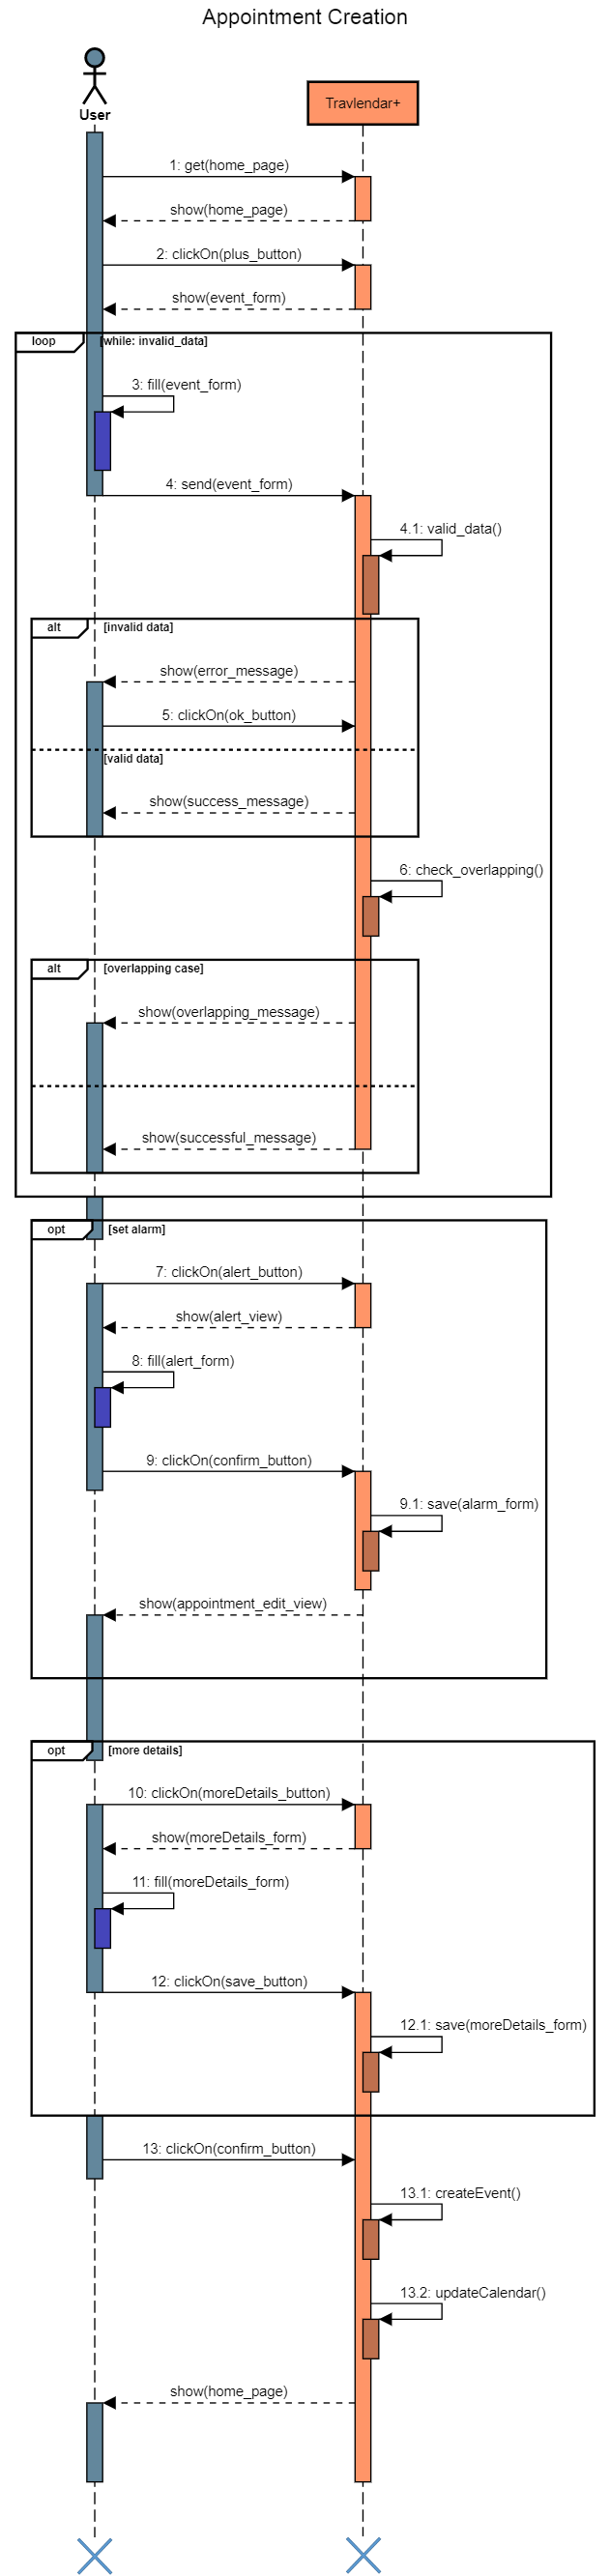
\includegraphics[width=0.50\textwidth]{Images/SequenceDiagram/AppointmentCreation.png}}%
	\end{minipage}
\end{figure}
\clearpage

\subsubsection{Appointment editing}
\begin{figure}[!h]
	\centering
	\begin{minipage}[b]{0.75\textwidth}
		\makebox[\textwidth][c]{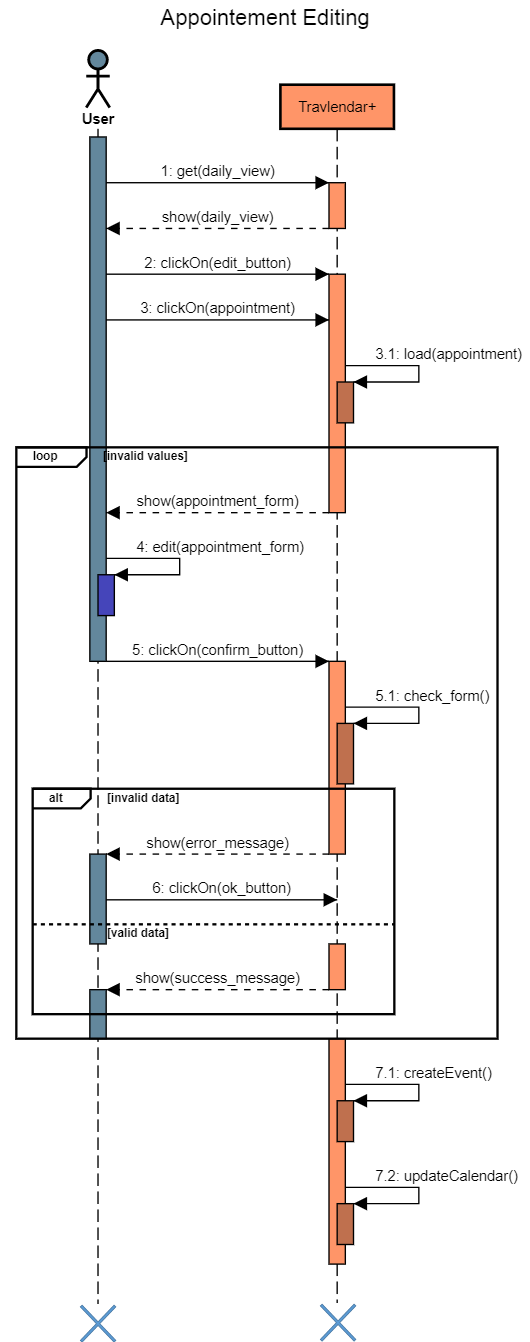
\includegraphics[width=0.50\textwidth]{Images/SequenceDiagram/AppointementEditing.png}}%
	\end{minipage}
\end{figure}
\clearpage

\subsubsection{Appointment deletion}
\begin{figure}[!h]
	\centering
	\begin{minipage}[b]{0.75\textwidth}
		\makebox[\textwidth][c]{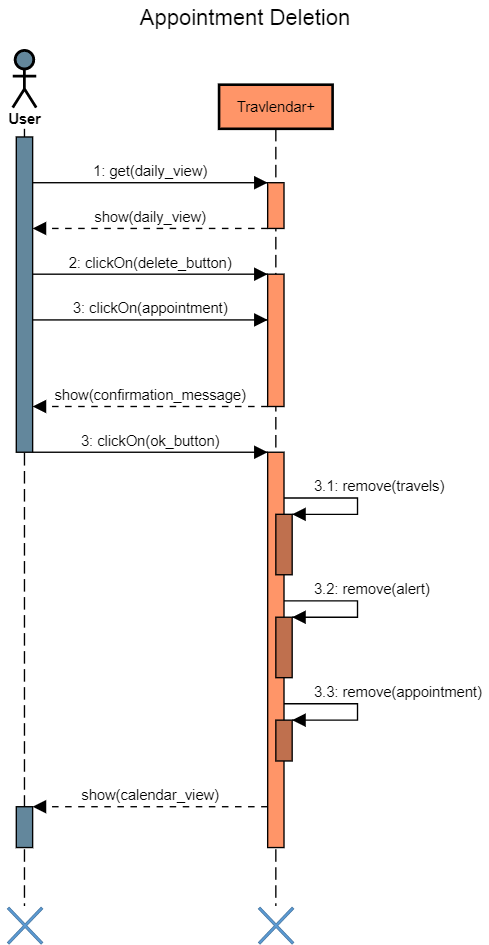
\includegraphics[width=0.50\textwidth]{Images/SequenceDiagram/AppointmentDeletion.png}}%
	\end{minipage}
\end{figure}
\clearpage

\subsubsection{Alert editing}
\begin{figure}[!h]
	\centering
	\begin{minipage}[b]{0.75\textwidth}
		\makebox[\textwidth][c]{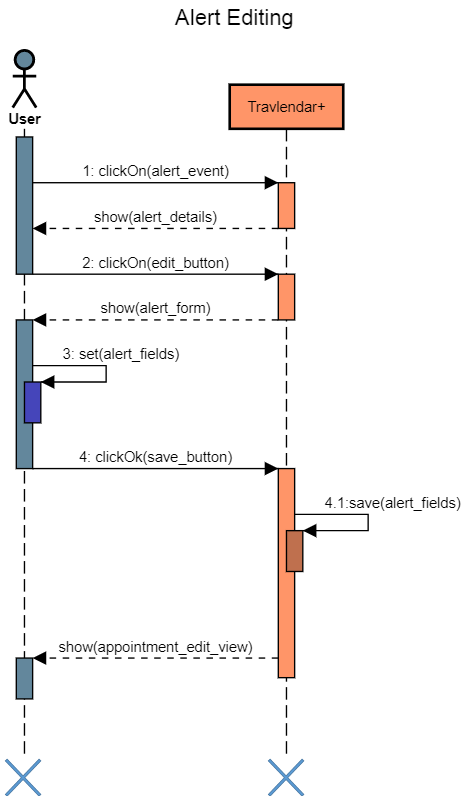
\includegraphics[width=0.50\textwidth]{Images/SequenceDiagram/AlertEditing.png}}%
	\end{minipage}
\end{figure}
\clearpage

\subsubsection{Alert deletion}
\begin{figure}[!h]
	\centering
	\begin{minipage}[b]{0.75\textwidth}
		\makebox[\textwidth][c]{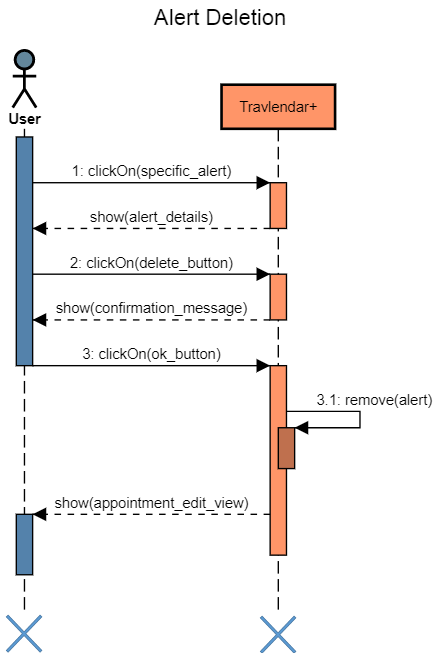
\includegraphics[width=0.50\textwidth]{Images/SequenceDiagram/AlertDeletion.png}}%
	\end{minipage}
\end{figure}
\clearpage

\subsubsection{Scheduling and view travels}
\begin{figure}[!h]
	\centering
	\begin{minipage}[b]{0.75\textwidth}
		\makebox[\textwidth][c]{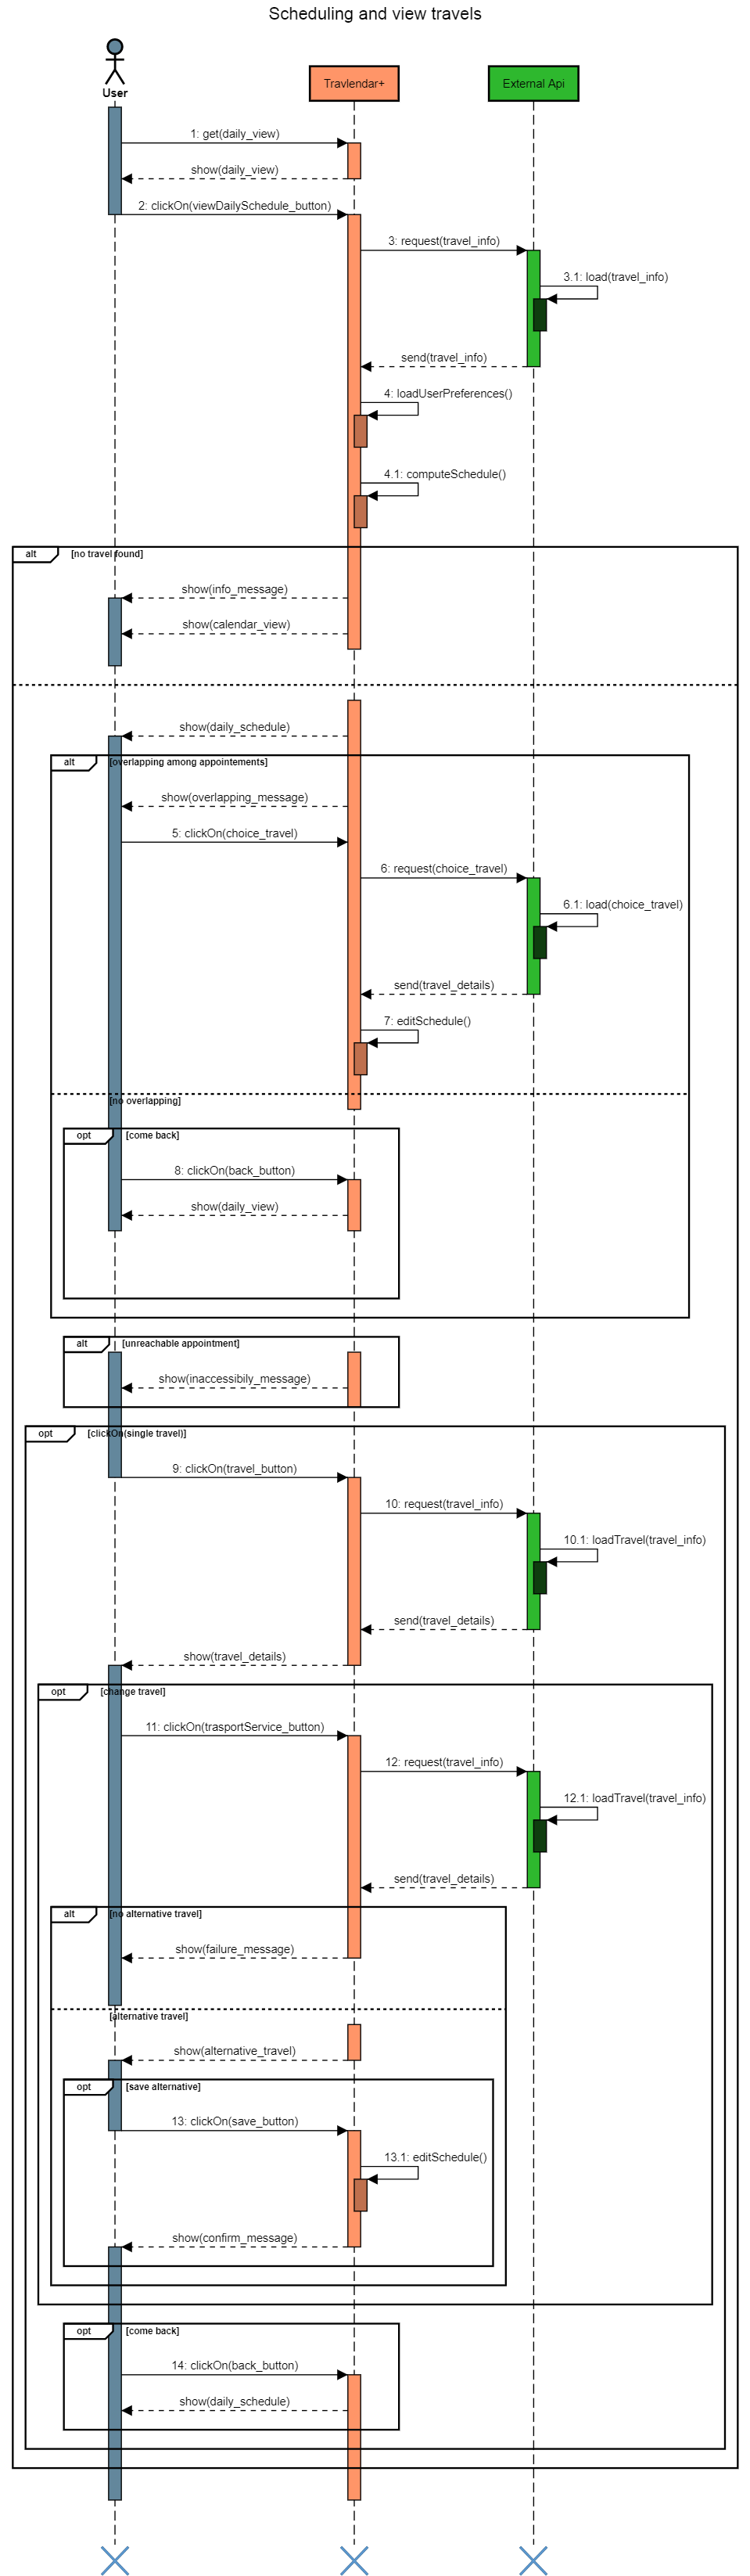
\includegraphics[width=0.50\textwidth]{Images/SequenceDiagram/SchedulingAndViewTravels.png}}%
	\end{minipage}
\end{figure}
\clearpage

\subsubsection{View and edit movements}
\begin{figure}[!h]
	\centering
	\begin{minipage}[b]{0.75\textwidth}
		\makebox[\textwidth][c]{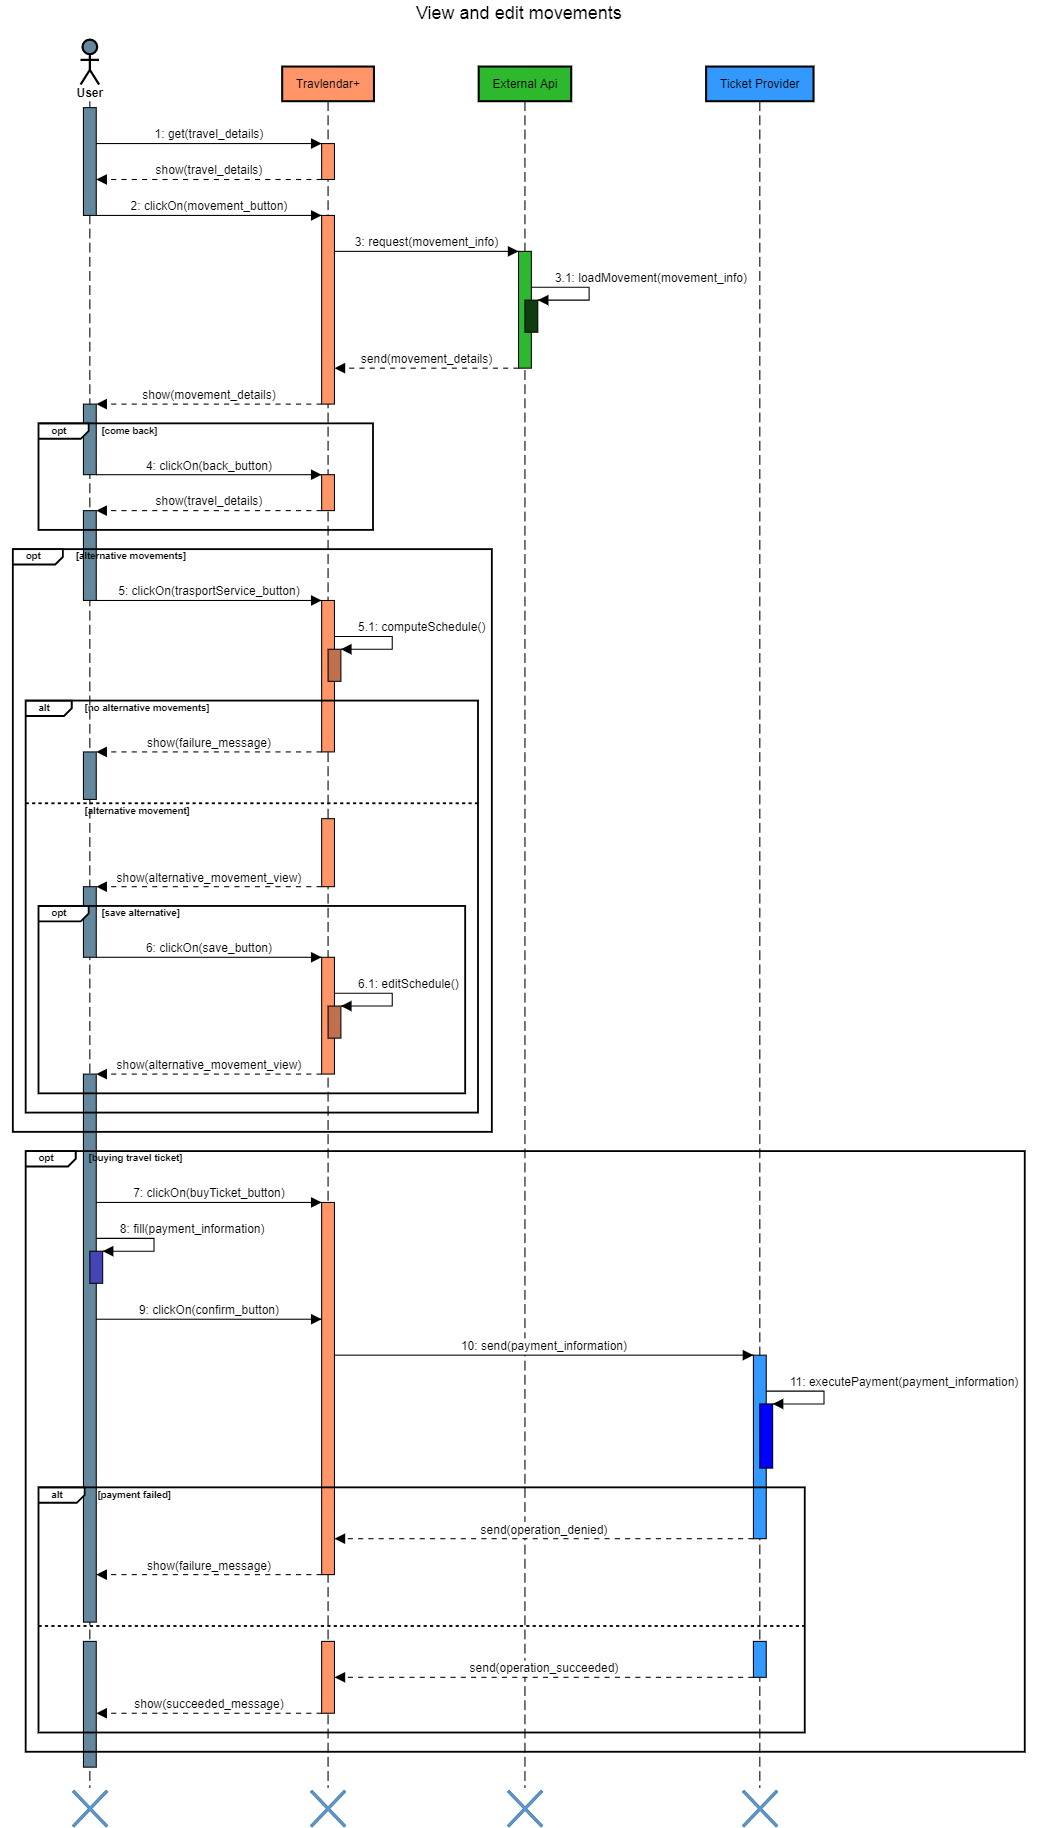
\includegraphics[width=0.50\textwidth]{Images/SequenceDiagram/ViewAndEditMovements.png}}%
	\end{minipage}
\end{figure}
\clearpage

\subsection{Activity diagram}
\subsubsection{Create appointment}
\begin{figure}[!h]
	\centering
	\begin{minipage}[b]{1\textwidth}
		\makebox[\textwidth][c]{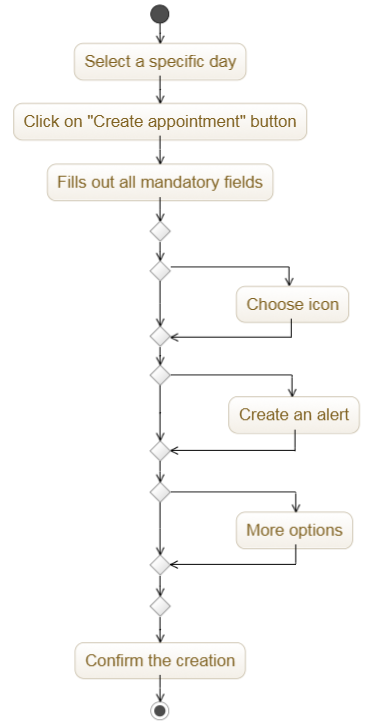
\includegraphics[width=0.50\textwidth]{Images/ActivityDiagram/CreateAppointment.png}}%
	\end{minipage}
\end{figure}
\clearpage

\subsubsection{Edit appointment}
\begin{figure}[!h]
	\centering
	\begin{minipage}[b]{1\textwidth}
		\makebox[\textwidth][c]{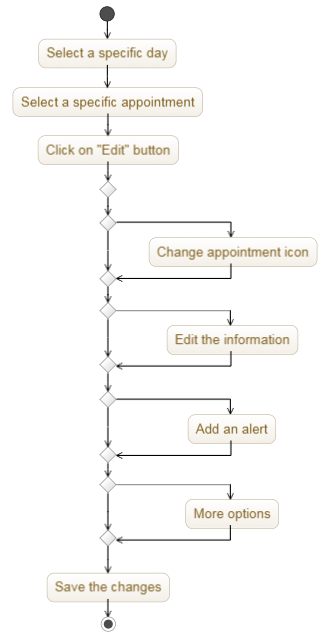
\includegraphics[width=0.50\textwidth]{Images/ActivityDiagram/EditEvent.png}}%
	\end{minipage}
\end{figure}
\clearpage

\subsubsection{Delete appointment}
\begin{figure}[!h]
	\centering
	\begin{minipage}[b]{0.8\textwidth}
		\makebox[\textwidth][c]{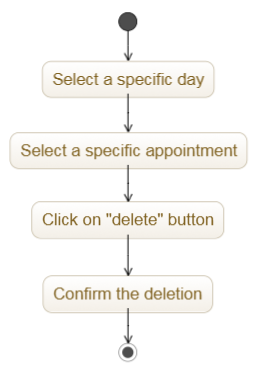
\includegraphics[width=0.50\textwidth]{Images/ActivityDiagram/DeleteEvent.png}}%
	\end{minipage}
\end{figure}

\subsubsection{Create alert}
\begin{figure}[!h]
	\centering
	\begin{minipage}[b]{1\textwidth}
		\makebox[\textwidth][c]{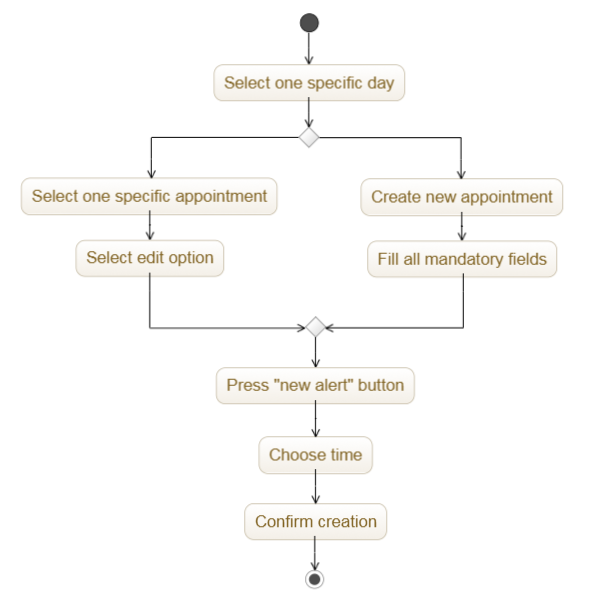
\includegraphics[width=0.50\textwidth]{Images/ActivityDiagram/CreateAlert.png}}%
	\end{minipage}
\end{figure}
\clearpage

\subsubsection{Edit travel}
\begin{figure}[!h]
	\centering
	\begin{minipage}[b]{1\textwidth}
		\makebox[\textwidth][c]{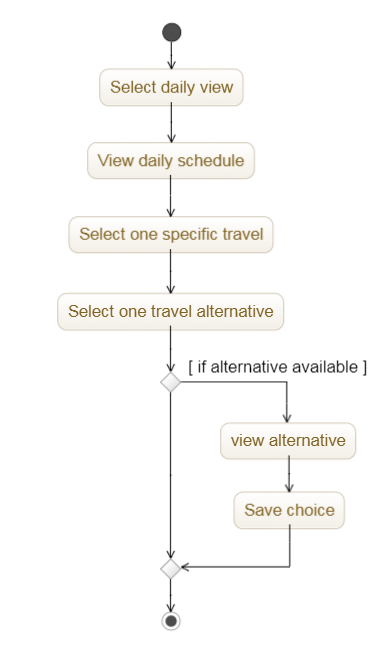
\includegraphics[width=0.50\textwidth]{Images/ActivityDiagram/EditTravel.png}}%
	\end{minipage}
\end{figure}
\clearpage

\subsubsection{Movement alternative}
\begin{figure}[!h]
	\centering
	\begin{minipage}[b]{1\textwidth}
		\makebox[\textwidth][c]{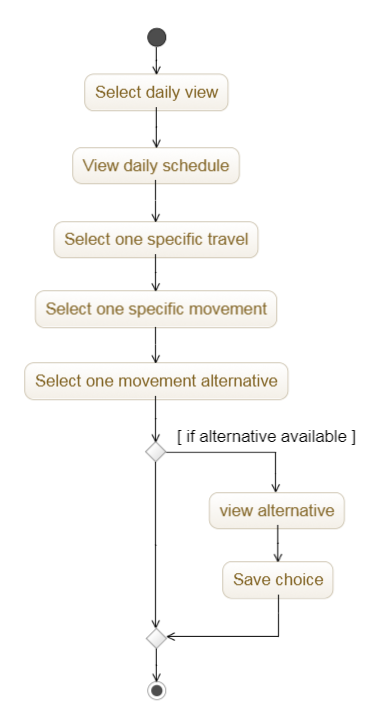
\includegraphics[width=0.50\textwidth]{Images/ActivityDiagram/MovementAlternative.png}}%
	\end{minipage}
\end{figure}
\clearpage

\subsubsection{Buy ticket}
\begin{figure}[!h]
	\centering
	\begin{minipage}[b]{1\textwidth}
		\makebox[\textwidth][c]{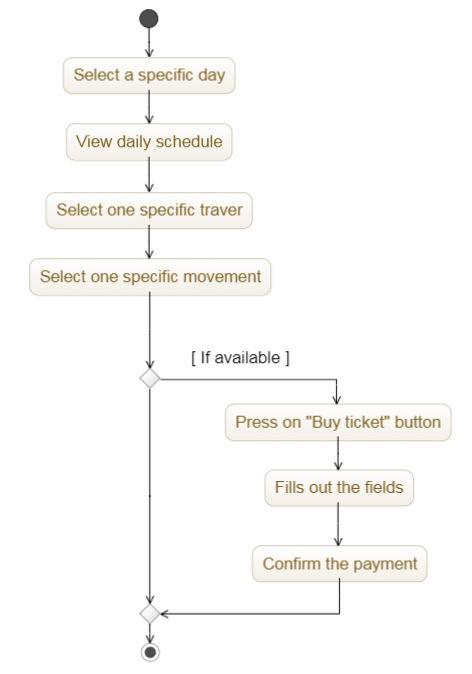
\includegraphics[width=0.50\textwidth]{Images/ActivityDiagram/BuyTicket.png}}%
	\end{minipage}
\end{figure}
\clearpage
